\documentclass[a4paper, oneside]{article}
\usepackage[english, russian]{babel}

\usepackage{fontspec}
\setmainfont[
  Ligatures=TeX,
  Extension=.otf,
  BoldFont=cmunbx,
  ItalicFont=cmunti,
  BoldItalicFont=cmunbi,
]{cmunrm}
\usepackage{unicode-math}

\usepackage[bookmarks=false]{hyperref}
\hypersetup{pdfstartview={FitH},
            pdfauthor={Павел Соболев}}

\usepackage[lmargin=23mm]{geometry}

\usepackage[table]{xcolor}
\usepackage{booktabs}
\usepackage{caption}

\usepackage{graphicx}
\graphicspath{ {./figures/} }

\usepackage{sectsty}
\sectionfont{\centering}
\subsubsectionfont{\centering \vspace{-0.5em}\normalfont\itshape}

\newcommand{\npar}{\par\vspace{\baselineskip}}
\newcommand{\su}{\vspace{-0.5em}}
\newcommand{\sd}{\vspace{0.5em}}

\setlength{\parindent}{0pt}

\hypersetup{pdftitle={Астрофизическая практика: отчет по второй работе}}

\begin{document}

\section*{Работа №2: Определение постоянной Хаббла}
\subsubsection*{Выполнил: Павел Соболев}

\vspace{3em}

\subsection*{Задачи}

\begin{itemize}
  \setlength\itemsep{-0.1em}
  \item Получить спектр галактики в скоплении, используя моделируемый с помощью компьютера телескоп и спектрометр;
  \item Измерив длины волн линий H и K (Ca II) в спектре, определить Доплеровское смещение;
  \item Определить видимую звездную величину галактики;
  \item Вычислить расстояние, используя видимую и абсолютную величины;
  \item Определить значение постоянной Хаббла.
\end{itemize}

\subsection*{Ход выполнения и результаты}

В ходе работы с виртуальным телескопом и спектрометром были получены следующие данные:

\begin{table}[h]
  \centering
  \caption{Звездные величины и длины волн}
  \begin{tabular}{cccccc}
    \toprule
    Скопление &
    Код объекта &
    Зв. величина &
    K Ca II ($ \lambda, I $) &
    H Ca II ($ \lambda, I $) &
    G Band ($ \lambda, I $) \\
    \midrule
    Ursa Major II & uma2-1 & 16.87 & 4484.0, 0.465 & --- & --- \\
    \arrayrulecolor{black!40}
    \midrule
    Ursa Major I & uma1-3 & 14.49 & 4130.0, 0.315 & 4167.0, 0.315 & --- \\
    \midrule
    Coma Berenices & Coma1 & 12.30 & 4012.0, 0.255 & 4048.0, 0.265 & 4391.0, 0.605 \\
    \midrule
    Bootes & Boot1 & 16.52 & 4445.0, 0.465 & 4485.0, 0.485 & --- \\
    \midrule
    Corona Borealis & CrBor1 & 15.08 & 4209.0, 0.330 & 4246.0, 0.345 & --- \\
    \midrule
    Sagittarius & GAS & 10.98 & 3973.0, 0.235 & 4008.0, 0.255 & 4348.0, 0.600 \\
    \arrayrulecolor{black}
    \bottomrule
  \end{tabular}
\end{table}

Пропуски означают отсутствие линии в наблюдаемом участке спектра. \npar

Звездные величины были пересчитаны в расстояния согласно

$$
M = m + 5 - 5 \lg{D}, \; \Longrightarrow \; \lg{D} = (m - M + 5) \, / \, 5,
$$
\su

где абсолютная звездная величина $M$ полагается равной $-22^m$ для всех объектов. \npar

Замеры линий были пересчитаны в доплеровские смещения и скорости согласно

$$
\Delta \lambda = \lambda_{\text{измер.}} - \lambda_{\text{станд.}},
$$
\su

\su\su
$$
v_K = c \frac{\Delta \lambda_K}{\lambda_{K, \text{станд.}}}, \quad
v_H = c \frac{\Delta \lambda_H}{\lambda_{H, \text{станд.}}},
$$
\sd

где $ \lambda_{K, \text{станд.}} = 3933.67 $ \AA, $ \lambda_{H, \text{станд.}} = 3968.847 $ \AA, $ c = 299792.458 $ км/с. \npar

\newpage

Результаты вычислений:

\begin{table}[h]
  \centering
  \caption{Расстояния и скорости}
  \begin{tabular}{cccc}
    \toprule
    Скопление &
    Код объекта &
    Расстояние &
    Скорость \\
    \midrule
    Ursa Major II & uma2-1 & 594.29 & 41941.69 $\pm$ 76.21 \\
    \arrayrulecolor{black!40}
    \midrule
    Ursa Major I & uma1-3 & 198.61 & 14965.22 $\pm$ 53.65 \\
    \midrule
    Coma Berenices & Coma1 & 72.44 & 5974.31 $\pm$ 53.65 \\
    \midrule
    Bootes & Boot1 & 505.83 & 38978.89 $\pm$ 53.65 \\
    \midrule
    Corona Borealis & CrBor1 & 260.62 & 20959.28 $\pm$ 53.65 \\
    \midrule
    Sagittarius & GAS & 39.45 & 2977.45 $\pm$ 53.65 \\
    \arrayrulecolor{black}
    \bottomrule
  \end{tabular}
\end{table}

Построенная на основе этих данных диаграмма Хаббла выглядит следующим образом:

\begin{figure}[h]
  \centering
  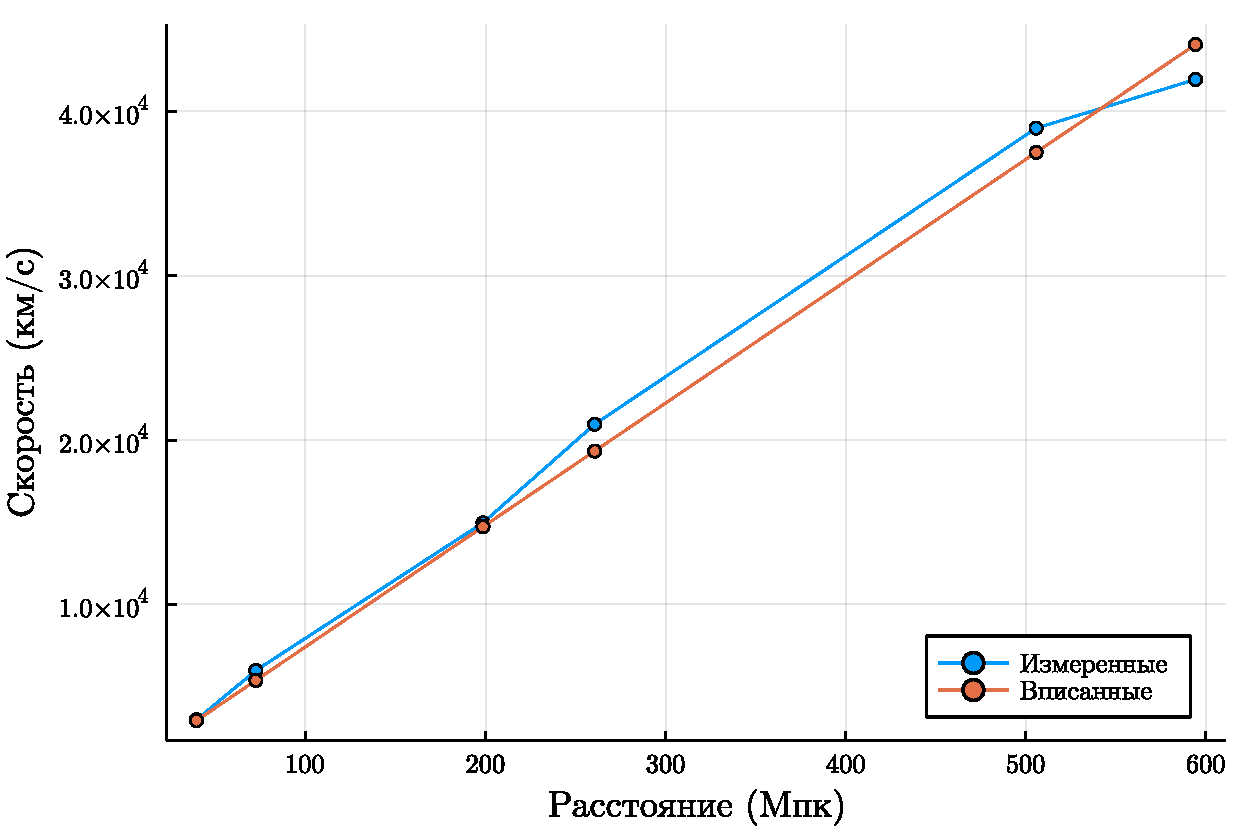
\includegraphics[scale=0.5]{result}
  \caption{Диаграмма Хаббла}
\end{figure}

Коэффициент вписанной прямой (он же постоянная Хаббла) равен $ 74.151 \pm 0.077 $ км/c/Мпк.

\end{document}